\documentclass{article}
\usepackage[homework]{ahmeds}

\initialize{1}

\begin{document}

\start{Ahmed Shakil}{Math H185}{Review Sheet}

\tableofcontents

\newpage

\section{Tools and Tricks}
\begin{misc}{Properties of the modulus}{}
    \begin{align*}
        z\overline{z} &= \left\lvert z \right\rvert ^{2} \\
        \overline{z\cdot w}&= \overline{z} \cdot \overline{w}  \\
        \left\lvert z\cdot w \right\rvert &= \left\lvert z \right\rvert \cdot \left\lvert w \right\rvert 
    \end{align*}
    
    \end{misc}
    
    \begin{misc}{\( z^n = \omega  \) }{}
    Let \( \omega = re^{i \theta } \), with \( r>0 \), and \( n>0 \).
    \begin{align*}
        z^n &= \omega \\
        z &= \sqrt[n]{r} e^{i (\frac{\theta + 2\pi k}{n}) }, k \in \left\{ 0,1, \dots , n - 1 \right\} 
    \end{align*}
    
    \end{misc}
    
    \begin{misc}{Standard nonholomorphic functions}{}
    The following functions are \( \mathbb{C} \to \mathbb{C}  \) and are not holomorphic at any point in the complex plane. 
    
    \begin{align*}
        f_1(z) &= |z|\\
        f_2(z) &= \overline{z} 
    \end{align*}
    
    \end{misc}
    
    \begin{misc}{Expansion of \( e^z \) }{}
        This is the Taylor expansion of the exponential function about \( z = 0 \).  
    \begin{align*}
        e^z = \sum_{n \geq 0} \frac{z^n}{n!}
    \end{align*}
    
    \end{misc}
    
    \begin{misc}{Some useful limits}{}
    \begin{align*}
        \lim_{n \to \infty} \sqrt[n]{n} = 1
    \end{align*}
    
    \end{misc}
    
    \begin{misc}{Bounding the \( \sin \) function}{}
    \begin{align*}
        \sin \theta \geq \frac{2\theta }{\pi }, \ \ \theta \in \left[ 0, \frac{\pi}{2} \right]  
    \end{align*}

    \end{misc}
    \begin{thrm}{Weierstrass's Approximation Theorem}{}
        Any continuous function \( f(x) \) on \( [0,1] \) can be uniformly approximated by polynomials, meaning that one can find a sequence of polynomials \( p_{n} (x) \) converging uniformly to \( f(x) \) on \( [0,1] \).
        \end{thrm}
        
        \begin{thrm}{}{}
        If \( f:\mathbb{C} \to \mathbb{C}  \) is holomorphic and non-constant, then \( f(\mathbb{C} ) \) is dense in \( \mathbb{C}  \). 
        \end{thrm}

\newpage


\section{The Basics}

\begin{thrm}{Euler's Theorem}{}
    \begin{align*}
        e^{iz} = \cos (z) + i\sin (z)  
    \end{align*}
    
    \begin{proof}
    Follows from the Taylor series expansion formulas.
    \end{proof}
    
    \end{thrm}

    \begin{exmp}{Neighborhoods in \( \mathbb{C}  \) }{}
        Let \( z_0 \in \mathbb{C}  \) and \( 0<r\in \mathbb{R}  \).
        \[
            \overline{B_{r} (z_0) }\coloneqq \left\{ z \in \mathbb{C} : |z - z_0| \leq  r \right\}  
        \]
        is the closed ball of radius \( r \) around \( z_0. \) 
        
        Similarly, 
        \[
            B_{r} (z_0) \coloneqq \left\{ z\in \mathbb{C} : |z - z_0| <r \right\} 
        \]
        is the open ball of radius \( r \) around \( z_0. \)
        
        A subset \( U \subset \mathbb{C}  \) is open if \( \forall z \in U \), \( \exists r  \in \mathbb{R}_{>0}  \)  such that \( B_{r} (z) \subset U  \). 
        \end{exmp}
        
        It is important to note that a sequence \( \left\{ z_n = x_{n} + iy_{n}  \right\} \subset \mathbb{C}   \)  converges to \( z \in \mathbb{C} \) if and only if 
        \[
            \lim_{n \to \infty} x_{n} = x \text{  and  } \lim_{n \to \infty} y_{n} = y.
        \]

        \section{Complex Derivatives}

        Let \( U \) be an open subset of \( \mathbb{C} \) and \( f: U \to \mathbb{C}  \) be a function. 
        
        \begin{defn}{Holomorphic at a point}{}
        We say \( f \) is holomorphic at some point \( z_0 \) if \( \lim_{h \to 0} \frac{f(z_{0} + h )- f(z)}{h}  \) exists in \( \mathbb{C} \). Equivalently it is holomorphic at \( z_0 \) if the following limit exists
        \[
            \lim_{z_0 \to z} \frac{f(z)- f(z_0)}{z - z_{0}} .
        \]
        If these limits exists, then we denote the value as \( f^\prime (z_0) \).
        \end{defn}
        
        \begin{rmk}{About holomorphic functions}{}
        Holomorphicity is a property which is quite a lot stronger than typically differentiability in the real number world. Holomorphicity means we demand the limit to be the same along any path of approach to a particular point. A common example of a function which is not holomorphic due to limits not being consistent along different paths of approach is the conjugation function: \( f(z) = \overline{z} . \) This function is not holomorphic at any point in the complex plane. 
        
        \hfill
        
        Some cool properties of holomorphic functions
        \begin{itemize}
            \item If a function is holomorphic at a point, then it is automatically infinitely complex differentiable at this particular point
            \item If \( f,g \) are holomorphic on a connected \( U \subset \mathbb{C}  \) and \( f = g \) on a line segment, then \( f = g  \) on all of \( U \) 
        \end{itemize}
        \end{rmk}
        
        Something important to note about complex differentiation is that the typical differentiation rules from the real numbers hold. So things like the product, quotient, chain, and addition rules hold. Also, the rules for differentiating polynomials are the same as well. Ratio of polynomials are holomorphic at all points in the complex plan other than the points at which the denominator is equal to \( 0 \).

\section{Power Series}

A power series is an expression of the following form:
\[
    \sum_{n\geq 0} a_{n} z^n = a_{0} + a_{1}z + a_2 z^{2} + \dots   
\]

\begin{rmk}{Manipulating power series}{}
Addition:
\[
    (\sum_{n\geq 0} a_{n} z^n )+(\sum_{n \geq 0} b_{n} z^n) = \sum_{n\geq 0} (a_{n} + b_{n} )z^n 
\]

Multiplication:
\[
    (\sum_{n\geq 0}a_{n} z^n )(\sum_{n\geq 0} b_{n} z^n ) = \sum_{n\geq 0}(\sum_{j + k = n}a_{j} b_{k}  )z^n 
\]
\end{rmk}


A power series defines a function when it converges. Recall that we say \( \sum z_{n}   \) converges absolutely if \( \sum |z_{n} | \) converges. Also recall that absolute convergence implies convergence.

\begin{defn}{Radius of Convergence}{}
   For a power series \( \sum_{n\geq 0}  a_{n} z^n\), we define the radius of convergence as 
   \[
       r\coloneqq (\limsup_{n \to \infty} |a_{n} |^\frac{1}{n})^{-1} 
   \]
   \end{defn}
\begin{thrm}{Convergence of power series}{}
    \begin{enumerate}[]
        \item If \( |z| < r \), then the power series converges absolutely.
        \item If \( |z| >r \), then the power series diverges. 
        \item If \( |z| = r \), then more examination is required, the series could converge or diverge. 
    \end{enumerate}
\end{thrm}


\subsection{Differentiation of Power Series}

For \( z_0 \in \mathbb{C}  \), a power series centered at \( z_0 \) is an expression
\[
    f(z) \coloneqq \sum_{n\geq 0} a_{n}(z - z_0)^n 
\]

Once again, it's radius of convergence is given by \( r\coloneqq (\limsup_{n \to \infty} |a_{n} |^\frac{1}{n})^{-1} \), and it converges absolutely for \( |z - z_0| < r \).

\begin{thrm}{}{}
\begin{enumerate}[]
    \item $f(z)$ is holomorphic at all \( z \in  B_{r} (z_0) \), and 
    \item \( f'(z) = \sum_{n\geq 0} na_{n} z^{n- 1}   \) is also holomorphic on \( B_{r} (z_0) \) with the same radius of convergence. 
\end{enumerate}
\end{thrm}

\begin{defn}{Analytic function}{}
A function \( f: U \to \mathbb{C}  \) on an open subset \( U \subset \mathbb{C}  \) is analytic if for every \( z_0\in  U \), \( \exists \ r>0  \) such that \( f \) agrees with an absolutely convergent power series on \( B_{r}(z_0) \). 
\end{defn}

Examples of analytic functions are \( \sin (z) \) and \( \cos (z) \). 

\subsection{Cauchy-Riemann Equations}

As we mentioned before \C{} is basically isomorphic to \R{2} when viewed as metric spaces. However, in terms of differentiability they are not the same. Now say we have some open \( \Omega \subset \mathbb{C} \) and \( f: \Omega \to \mathbb{C}  \). We can write \( f \) as the following function:
\begin{align*}
    f &= u + iv, \text{\quad where } \\ 
    u &= \Re (f): \Omega \to \mathbb{C} \\
    v &= \Im (f): \Omega \to \mathbb{C} 
\end{align*}

Using this, given some \( z = x + iy \), we view \( u(z) = u(x,y) \) and the same goes for \( v \) as well. 

\begin{thrm}{Cauchy-Riemman Equations}{}
If \( f \) is holomorphic at \( z _0 \), then 
\begin{align*}
    \frac{\partial u}{\partial x}(z_0) &= \frac{\partial v}{\partial y}(z_0) \\
    \frac{\partial u}{\partial y}(z_0) &= - \frac{\partial v}{\partial x}(z_0) \\
\end{align*}
These are called the Cauchy-Riemann equations. 
    \tcbline

    \begin{proof}
    \begin{align*}
        \lim_{{\underset{\in \mathbb{R}}{x}  \to 0}} = \frac{f(z_0 + x)- f(z_0)}{x} = f& ^\prime(z_0) = \lim_{\underset{\in \mathbb{R} }{y}  \to 0} \frac{f(z_0+ iy) - f(z_0)}{iy} \\ 
        \frac{\partial f}{\partial x}(z_0) &= \frac{1}{i}\frac{\partial f }{\partial y}(z_0) \\
        \frac{\partial u}{\partial x} (z_0) + i \frac{\partial v}{\partial x} (z_0) &= \frac{1}{i}(\frac{\partial u}{\partial y} (z_0) + i\frac{\partial v}{\partial y} (z_0))  \\
        \implies  &\begin{cases}
        \frac{\partial u}{\partial x}(z_0) &= \frac{\partial v}{\partial y}(z_0) \\
        \frac{\partial u}{\partial y}(z_0) &= - \frac{\partial v}{\partial x}(z_0) \\
        \end{cases}
    \end{align*}
    
    \end{proof}
    \tcbline

    It is also important to note that there exists a converse result. If \( f \) is in \( C^1 \), meaning \( \frac{\partial u}{\partial x} , \frac{\partial u}{\partial y} , \frac{\partial v}{\partial x} , \frac{\partial v}{\partial y}  \) all exist and are continuous, and the Cauchy-Riemann equations hold, then \(  f \) is holomorphic. 
\end{thrm}

The partial derivative matrix of a holomorphic function has the following special form:
\begin{align*}
    \begin{bmatrix}
        \frac{\partial u}{\partial x}  & \frac{\partial u}{\partial y}   \\
         \frac{\partial v}{\partial x} &  \frac{\partial v}{\partial y}  \\
    \end{bmatrix} = \begin{bmatrix}
        a &   b \\
        -b &  a \\
    \end{bmatrix}
\end{align*}

It is important to note that holomorphic functions are conformal mappings, meaning they infinitesimally preserve angles or scale them to 0.



\section{Integrating Over Curves}

Integrating in complex analysis in the most basic sense amounts to the following.
\[
    \int f(z) dz = \int \Re (f(z))dz + \int \Im (f(z)) dz
\]

\subsection{Curves}

The idea is the connect \( \int _\gamma  \) to \( \int _a^b \) using substitution, where \( \gamma  \) is a curve.

\begin{defn}{Parametrized Curve}{}
A parametrized curve is a continuous function
\[
    \gamma (t): [a,b] \subset \mathbb{R} \to \mathbb{C} 
\]
\end{defn}

We say a curve \( \gamma  \) is piecewise smooth if we can divide the domain \( [a,b] \) into finitely many subintervals on which \( \gamma  \) is smooth (i.e. infinitely differentiable).

\subsubsection{Integration on Parametrized Curves}

\begin{thrm}{$U$-substitution}{}
If \( \gamma : [a,b] \to \mathbb{C}  \) is piecewise-smooth, and \( f \) is defined on the image of \( \gamma \), then 
\[
    \boxed{\int _\gamma  f(z) dz = \int ^b_a f(\gamma (t))\gamma ^\prime (t) dt.} 
\]
\end{thrm}

An important property to note is that reversing the orientation of the curve is equal to taking the negative of the original curve. The reverse of \( \gamma  \) is defined as follows.
\[
    \gamma ^-(t ) = \gamma (b + a - t)
\]
Then \(- \int _{\gamma ^-} f(z) dz = \int _\gamma f(z) dz \) (this is proved using a substition and change of variables). As a matter of definitions it is important to note that we refer to an antiderivative as a primitive, these terms should be taken as one and the same. 

\begin{thrm}{Fundamental Theorem of Calculus}{}
    \[
        \int_\gamma f(z) dz = F(\gamma (b)) - F(\gamma (a))
    \]
    \tcbline
    \emph{Corollary:}
    
    If \( \gamma : [a,b]\to \mathbb{C}  \) is a closed loop, i.e. \( \gamma (a) = \gamma (b) \), then 
    \[
        \int _\gamma f(z) dz = F(\gamma (b)) - F(\gamma (a)) = 0
    \]
    \end{thrm}

    \begin{exmp}{The most fundamental example}{}
        Say \( f(z) = z^n \) and \( n \in \mathbb{Z}  \). Consider the curve \( \gamma (t)= re^{it}  \) where \( r \in \mathbb{R} _{>0} \) and \( t \in [0, 2\pi ] \).
        Calculate \( \int _\gamma f(z) dz \) for all \( n \in \mathbb{Z}  \).
        \tcbline
        
        \begin{align*}
            \int _\gamma f(z) dz &= \int_{0}^{2\pi} r^n e^{nit} (rie^{it}) dt \\ 
            &= ir^{n+ 1} \int _0^{2\pi } e^{(n + 1)it} dt
        \end{align*}
        
        \underline{If \( n\neq -1 \):} A primitive for \( e^{(n + 1)it} \)  is \( \frac{1}{(n + 1)i} e^{(n + 1)it}\).
        
        \begin{align*}
            \implies \boxed{\int_\gamma f(z) dz = 0 \tag{$n \neq - 1$}} 
        \end{align*}
        
        \underline{If \( n = -1 \):}
        \begin{align*}
            ir^{0} \int _0^{2\pi } e^{(0)it} dt = 2\pi i\\
            \implies \boxed{\int_\gamma f(z) dz = 2\pi i \tag{$n = - 1$}}
        \end{align*}
        
        \underline{Conclusion:}
        
        \begin{align*}
            \int _{\partial B_r(0)}z^n dz = \begin{cases}
                0 \ \ &n\neq - 1 \\
                2\pi i \ \ &n = - 1
            \end{cases}
        \end{align*}
        
        
        \end{exmp}
        

        \subsubsection{Cauchy's Theorem}

        A boundary of a subset \( \Omega \subset \mathbb{C}  \) is \( \overline{\Omega }\setminus  \Omega ^\circ  \). Basically the boundary is the points in the closure of a set which is not in the interior of the set. 
        
        An important thing to note about substitutions:
        If \( g(z) \) is holomorphic on an open neighborhood of \( \gamma  \) 
        \begin{align*}
            \int _\gamma f(g(z)) dz = \int _{g \circ \gamma } f(z) g^\prime (z) dz.
        \end{align*}
        
        \begin{thrm}{Goursat's Theorem}{}
            If \( f(z) \) is holomorphic on a neighborhood containing \( \Delta   \) then 
            \[
                \int _\Delta f(z) dz = 0.
            \]
            \tcbline
            The summary of the proof is as follows, subdivide the original triangle to estimate the original integral. Eventually the sequence of triangles, where you take the supremum at each divsion and construct an estimate, has a limit point. Use linear approximations to conclude. 
            \end{thrm}

        \begin{thrm}{Cauchy's Theorem}{}
        If \( U \subset \mathbb{C}  \) is an open set and has a piecewise-smooth boundary, and \( f(z) \) is holomorphic on a domain containing \( \overline{U}  \), then
        \[
            \int _{\partial U } f(z) dz = 0.
        \]
        
        This is the most fundamental and remarkable tool in complex analysis.
        \tcbline
        It is important to note that we take this as a consequence of Goursat's theorem. Estimate the set by a polygon, divide it up into a sum of integrals over triangles, then apply Goursat's theorem. 
        \end{thrm}



        Contour manipulation is an important technique to note. This is because to calculate an integral on a curve, we can deform that curve through a domain where our function is holomorphic in order to calculate our desired result. 

        \begin{thrm}{Cauchy's formula}{}   
        Suppose we have \( f: \Omega \subset \mathbb{C}  \to \mathbb{C}  \) which is defined on an open set as the domain, and is holomorphic. Let \( z_0 \in \Omega  \) and \( r > 0 \) such that \( B_r(z_0) \subset \Omega  \). Then for all \( z \in B_ r(z_0), \) we have 
        \[
            f(z) = \frac{1}{2\pi i}\int _{\partial B_r(z_0)}\frac{f(w)}{w - z}dw. 
        \]
        
        \tcbline
        \begin{proof}
        We relegate the proof to the lecture notes as it is quite technical. 
        \end{proof}
        
        \end{thrm}


        \begin{cor}{Infinite differentiability}{}
            As a result of Cauchy's formula we have that wherever \( f \) is holomorphic it is infinitely differentiable. 
            
            We can differentiate Cauchy's formula to derive the following more general formula for higher order derivatives:
            
            \begin{align*}
                \boxed{f^{(n)}(z) = \frac{n!}{2\pi i}\int _{\partial B_r(z_0) } \frac{f(w)}{(w - z)^{n+ 1} } dw }
            \end{align*}
            
            \end{cor}
            
            \begin{lem}{Jordan's Lemma}{}
            Let \( f(z) = e^{iaz}g(z)  \)  where \( z \in \mathbb{C} \) and \( a > 0 \).
            
            Then
            \[
                \left\lvert \int _\gamma f(z) dz \right\rvert \leq \frac{\pi}{a}\sup _{\gamma }\left\lvert g(z) \right\rvert .
            \]
            Note that the curve is a semicircle with \( R \) as the radius.
            \end{lem}
            \begin{thrm}{}{}
                If \( f \) is holomorphic on a ball \( B_r(z_0) \) where \( z_0 \in \mathbb{C}  \) and \( r>0 \), then \( f \) has a primitive on \( B_r(z_0) \).
                \end{thrm}
                
                \begin{defn}{Homotopic Curves}{}
                Say we are given two parametrized curves (where \( U \subset \mathbb{C}  \) is an open set)
                \begin{align*}
                    \gamma _0: \left[ a,b \right] \to U \\
                    \gamma _1: \left[ a,b \right] \to U \\
                \end{align*}
                 where 
                \begin{align*}
                    \gamma _0(a) = \gamma_1(a) = z_a \\
                    \gamma _0(b) = \gamma _1(b) = z_b.
                \end{align*}
                We say \( \gamma _0  \) and \( \gamma _1 \) are homotopic in \( U \) if there exists a jointly continuous \( \gamma _s (t) \) where \( s \in [0, 1] \) and \( t \in \left[ a,b \right]  \) such that \begin{align*}
                    \gamma _s(a) = z_a \quad \forall s\\
                    \gamma _s(b) = z_b \quad \forall s\\
                    \gamma _s (t) \mid _{s = 0} = \gamma _0(t) \\
                    \gamma _s (t) \mid _{s = 1} = \gamma _1(t) \\
                \end{align*}
                
                \end{defn}
                \begin{defn}{Simply Connected}{}
                    We say \( U \) is simply connected if any two curves \( \gamma _0 \) and \( \gamma _1 \) in \( U \) with the same end points are homotopic in \( U \). 
                    \end{defn}

                    \begin{thrm}{Equivalence of Homotopic Curves}{}
                        If \( f \) is holomorphic on a open subset \( U \subset \mathbb{C}  \) where \( \gamma _0 \) and \( \gamma _1 \) are homotopic in \( U \), then 
                        \[
                            \int _{\gamma _0}f(z) dz = \int _{\gamma _1}f(z) dz.
                        \]
                        \end{thrm}
                        
                        \begin{thrm}{Existence of Primitives}{}
                        Any holomorphic function \( f \) on a simply connected domain \( U \subset \mathbb{C}  \) has a primitive \( F \) on \( U \). 
                        \end{thrm}
\section{The Riemann Sphere}

\begin{defn}{One-point compactification}{}
    The one point compactification of \C{} is     
\( \hat{\mathbb{C}}  = \mathbb{C} \cup \left\{ \infty  \right\}   \), usually it is called "extended \C{} plane" or the "Riemann Sphere".
\end{defn}

\begin{rmk}{}{}
More generally, \( f: U \setminus \{z_0\}\to \mathbb{C}  \) is meromorphic if and only if \(f  \) extends continuously to \( \hat{f} : U \to  \widehat{\mathbb{C}}  \), and has a pole at \( z_0 \) if and only if \( \hat{f} (z_0) = \infty  \).  
\end{rmk}


\begin{defn}{Biholomorphism}{}
A function \( f: U \to V, \text{ where }  \  U \ \& \ V \in \mathbb{C}  \) is a homomorphism if \( f \) is:
\begin{itemize}
    \item holomorphic,
    \item bijection,
    \item and \( f^{-1}  \) is holomorphic.
\end{itemize}
This is the natural notion of isomorphism in complex geometry.  
\end{defn}
\begin{misc}{Slogan}{}
Biholomorphisms preserve all intrinsic notions of holomorphic functions, for example, orders of singularities, residues, etc. 
\end{misc}

\begin{defn}{}{}
If \( f \) has a removable singularity (or some other type of singularity), then \( F(z)\coloneqq f(\frac{1}{z}) \) has a removable singularity (or the same corresponding type of singularity). This inversion allows us to do complex analysis near infinity.  
\end{defn}

\begin{misc}{Strengthining of Liouville's Theorem}{}
Suppose \( f:\mathbb{C} \to \mathbb{C}  \) is holomorphic and \( \exists  N,c \) such that \( |f(z)| \leq c |z|^N \) for all \( z \) in a punctured neighborhood of infinity. Then \( f \) is a polynomial of degree at most \( N \).  
\tcbline
\begin{proof}
We want \( f^{(N + 1)} = 0. \) 

Cauchy's inequality gives us the following:

\[
    f^{(n)}(z_0) \leq \frac{n!}{r^n}  \sup _{z \in \partial B_{r}(z_0) }\left\lvert f(z) \right\rvert 
\]

Now we can take \( n = N + 1 \) and \( r \) which is appropriate. 

\begin{align*}
    \left\lvert f^{(N + 1)}(z_0) \right\rvert &\leq \frac{(N + 1)!}{r^{N+ 1} }c(|z_0|+ r)^N \to 0 \text{ as } r \to \infty  
\end{align*}

Hence, we are done. 
\end{proof}

\end{misc}
\begin{cor}{}{}
Let \( f: \mathbb{C} \to \mathbb{C}  \) be a holomorphic function with a pole at \( \infty  \). Then \( f \) is a polynomial. 

\tcbline

\begin{proof}
We want to show that \( f \) satisfies the hypothesis of the preceding theorem. Let \( F(z ) = f(\frac{1}{z}) \). Then \( F \) has a pole at \( 0 \). This implies the following
\begin{align*}
    F(z) = \sum_{k\geq - m}a_{k} z^k = \frac{a_ {- m}}{z^m} + \dots 
\end{align*}
So for \( |z| \) small enough we have that \( |F(z) |\leq c|\frac{1}{z^m}| \), however, this implies \( |f(z)| \leq c|z|^m \) for \( |z| \) large enough. From here we can apply the preceding result and hence we are done. 
\end{proof}

\end{cor}

\begin{defn}{}{}
A rational function is a ratio of polynomials
\[ f(z) = \frac{P(z)}{Q(z)}.  \]
\end{defn}


\begin{thrm}{}{}
Let \( f: \hat{\mathbb{C}} \to \hat{\mathbb{C}}  \) be holomorphic (meromorphic). Then \( f \) is a rational function. 

\tcbline
\begin{proof}
We know that \( \hat{\mathbb{C}}  \) is compact and the singularities of \( f \) are isolated, they are finite in number, say they occur at \( z_1, \dots , z_N \) and possibly \( z_ 0 = \infty  \). \( f \) has a pole at each \( z_{j}  \), which means there is some \( n_{j}  \) such that \( f(z)\times (z - z_{j} )^{n_{j} }  \) extends holomorphically to \( z_{j}  \). This implies \( f(z)\prod_{j\geq 1}(z - z_{j} )^{n_{j} }   \) is holomorphic on all of \C{}. Now based on the corollary above the pole at infinity implies \( P(z) = f(z)\prod_{j\geq 1}(z - z_{j} )^{n_{j} } \) is a polynomial. Hence, it follows that \( f \) is in the form \( f(z) = \frac{P(z)}{Q(z)}  \).  
\end{proof}


\end{thrm}

\section{The Argument Principle}

\begin{thrm}{}{}
Suppose \( f \) has a zero of order \( n \) at \( z_0 \) (positive or negative). Then \( \frac{f'(z)}{f(z)}  \) has a simple pole if \( n\neq 0 \), and \( \mathrm{Res}_{z_0}(\frac{f'(z)}{f(z)} ) = n  \text{ for all }    n  \). 

\tcbline
\begin{proof}
Near \( z_0 \), \( f(z) = (z - z_0)^{n}h(z)  \), where \( h(z) \) is holomorphic and nonvanishing. 
\begin{align*}
    \implies& f'(z) = n(z - z_0)^{n -1}h(z)+(z - z_0)^n h'(z)\\
    \implies& \frac{f'(z)}{f(z)} = \frac{n}{z - z_0}+\frac{h'(z)}{h(z)}   
\end{align*}

\end{proof}

\end{thrm}

\begin{thrm}{Argument Principle}{}
Let \( f \) be meromorphic on a neighborhood of \( \overline{U}  \). Then
\begin{align*}
    \frac{1}{2\pi i}\int _{\partial U} \frac{f'(z)}{f(z)} dz = \text{\# of zeros in } U  - \text{\# poles in } U 
\end{align*}
counted with multiplicity. 

\tcbline

\begin{proof}
We apply the residue theorem. The poles of \( f'/f \) are the zeros and poles of \( f \). When we plug these into the residue formula, using the previous theorem we arrive at the answer. 
\end{proof}

\end{thrm}
As a consequence we have the following theorem.

\begin{thrm}{Rouche's Theorem}{}
Suppose \( f \) and \( g \) are holomorphic on a neighborhood of \( U \). If \( |f(z)| > |g(z)| \ \forall z\in \partial U \), then \( f(z) \) and \( f(z) + g(z) \) have an equal number of zeros in \( U \) when counted with multiplicity. 

\tcbline 

\begin{proof}
For \( \lambda \in \left[ 0,1 \right]  \), let \( f_\lambda (z) = f(z) + \lambda g(z) \). 
Then \( f_\lambda  \) is holomorphic on a neighborhood of \( \overline{U}  \), and \( f_0 = f \) and \( f_1 = f + g \).

We now apply the argument principle to \( f_\lambda (z)  \) on \( \overline{U}  \). 
We claim that \( f_\lambda  \) has no zeros on \(  \partial U\).
To prove this, for that sake of contradiction suppose \( f_\lambda = 0 \) for some point on \( \partial U \). 

Then this means that \( f +\lambda g = 0 \implies |f| = \lambda |g|\), by our assumption this cannot be true. Hence, we have ourselves a contradiction. 

Now, based on this claim we can use the argument principle on \( f_\lambda  \). We only need to consider the zeros of \( f_\lambda  \) since it is holomorphic by assumption. 

Based on the argument principle we have that 
\begin{align*}
    \frac{1}{2\pi i}\int _{\partial U}\frac{f'_\lambda (z)}{f _\lambda (z)}dz = n_\lambda,  
\end{align*}
where \( n_\lambda  \)  is the number of zeros of \( f_\lambda  \) inside \( U \). Now the right hand side must be an integer while on the left hand side the integral continuously depends on \( \lambda  \). This means that \( n_0 = n_1 \), because if it didn't then by the IVT the equality would break since it would open up the possibility for the right hand side to be a non integer number, which obviously is not possible. 
\end{proof}

\end{thrm}

\begin{cor}{Fundamental Theorem of Algebra}{}
Let \( P(z) = z^n + a_{n - 1} z^{n - 1} + \dots + a_0  \) for some \( n > 0 \). 
Then \( P \) has \( n \) zeros in \( \mathbb{C}  \) when counted with multiplicity. 

\tcbline

\begin{proof}
For \( R \gg 1 \),

\[
  r^n > |a_{n - 1} |r^{n- 1}+ \dots + |a_0| \ \ \forall r \geq R   .
\]
Let \( f(z) = z^n \), \( g(z) = a_{n- 1}z^{n- 1} + \dots + a_0   \). Then \( |f(z)| > |g(z)|, \ \forall z \in \partial B_R(0) \). Then by Rouche's theorem \( f \) and \( f + g  \) have the same number of zeros in \( B_R(0)\) . Clearly, \( f \) has \( n \) zeroes in \( B_R(0) \). 
\end{proof}

\end{cor}

\subsection{The Open Mapping Theorem}

\begin{defn}{Open Map}{}
A continuous map is open if it sends open sets to open sets. 
\end{defn}

\begin{thrm}{The Open Mapping Theorem}{}
If \( f: U \to \mathbb{C}  \) is holomorphic and nonconstant, then \( f \) is an open map. 
\tcbline
\begin{proof}
We want to show \( f(U) \) is also an open set in \C{}, where \( f \) is holomorphic and nonconstant. 

Suppose \( w_0 = f(z_0) \) for some \( z_0 \in U\). This means that \( f(z) - w_0 \) has \( z_0 \) as a zero. 

Consider a \( w \) close to \( w_0 \); we want \( f(z) - w \) to also have some zero in \( U \). 

To show that this is the case, we can compare the holomorphic functions \( f(z) - w \) and \( f(z) - w_0 \). Notice that 
\[
    f(z) - w = (f(z)- w_0) + (w_0 - w).
\]

Let \( z_0 \in U\) be a zero of \( f(z) - w_0 \). Because \( U \) is open there exists some \( \delta > 0 \) such that \( B_\delta (z_0) \subseteq U \). 

\( f \) is also not a constant function, so \( f(z) - w_0 \) is not a constant zero, so \( z_0 \) is an isolated zero of the function \( f(z) - w_0 \).

We can make \( \delta > 0  \) even smaller so that on \(\overline{B_\delta (z_0)}   \), \( z_0 \) is the unique zero of \( f(z) - w_0 \). 

Suppose we define \(\epsilon >0   \) such that 
\[
    \epsilon  = \frac{1}{2}\inf _{z \in \partial B_\delta (z_0)}|f(z) - w_0|.
\]

We then have for any \( w \in B_{\epsilon }(w_0)  \) and \( z \in \partial B_\delta(z_0)  \) that 
\[
   |f(z) - (w_0)| \geq \inf _{z \in \partial B_\delta (z_0)}|f(z) - w_0| = 2\epsilon >\epsilon >|w - w_0| = |w_0 - w|.
\]

Applying Rouche's theorem on \( B_\delta (z_0) \), we can say that \( (f(z)- w_0) + (w_0 - w) = f(z) - w \)  has the same number of zeros as \( f(z) - w_0 \). 

Since \( f(z) - w_0 \) has a zero \( z_0 \), we know that \( f(z) = w \) also has a solution in \( B_\delta (z_0) \subseteq U \). This means that \( w \in f(U) \), and this \( B_{\epsilon }(w_0) \subseteq f(U)  \), since \( w \in B_{\epsilon }(w_0)  \) is arbitrary. This shows that \( w_0 \) is an interior point. 
\end{proof}
\end{thrm}

\subsection{Geometric interpretation of the argument principle}

Say we have some \( z = re ^{i \theta }  \), we denote the argument as \( \arg (z) = \theta\).

Recall the argument principle:

\begin{align*}
    \frac{1}{2\pi i}\int _{\partial U} \frac{f'(z)}{f(z)} dz = \text{\# of zeros in } U  - \text{\# poles in } U .
\end{align*}

Let's denote \( f'/f = \frac{d\log (f)}{dz} = \frac{d}{dz}(\log r + i \theta )    \). So the integral 
\[
    \frac{1}{2\pi i}\int _{\partial U} \frac{f'(z)}{f(z)} dz
\]
is trying to measure the change in the angle as \( f \) goes around \( \partial U \). So in this case the number of zeros is equal to how many times \( f(\partial U) \) winds around \( 0 \). This understanding applies to holomorphic functions. If the function is meromorphic just subtract the number of poles just like in the argument principle. 

Locally, given some choice for \( \log (z_0) \), we define \( \log (z) \) near \( z_0  \) by the following:
\begin{align*}
    \int _{z_0}^z \frac{1}{w}dw.
\end{align*}

Similarly, \( \log (f(z)) \) is not well defined, but we use the following to make it well defined:
\begin{align*}
    \frac{d}{dz}\log (f(z)) = \frac{f'(z)}{f(z)} .
\end{align*}

\begin{align*}
    \int _{\partial U}\frac{f'(z)}{f(z) - w_0} dz &\text{ "\( = \)" } \int   _{\partial U}\frac{d}{dz} \log (f(z) - w_0) \\
    &  \ = \text{"winding number of \( f(\partial U) \)" around \( w_0 \).  }
\end{align*}

\begin{lem}{}{}
Suppose \( f: U \to \mathbb{C}  \) is holomorphic and \( f'(z_0)\neq  0\). Then \( f \) is a local biholomorphism onto its image near \( z_0 \), i.e. there exists
\begin{align*}
    z_0 \in U' \subset U \to  V' \subset V\\
\end{align*}
where \( f: U' \to V' \) is bijective, and \( f^{-1}  \) is holomorphic. 

\tcbline

\begin{proof}

First we show \( f \) is locally injective near \( z_0 \), i.e. there exists an open set where \(z_0 \in  U'  \)  such that \( f \) is injective on \( U' \). 

Let \( w_0 = f(z_0) \). If we consider \( f(z) - w_0 \), this function has isolated zeros. Because of this on \( \partial B_{r} (z_0) \) we have \( |f(z) - w_0| \geq \epsilon > 0 \). Then for \( w \in B_\frac{\epsilon }{2}(w_0) \) we have \( |w - w_0| < \frac{\epsilon}{2}\). 

So the number of zeros of \( f(z) - w_0 \) equals 1 on \( B_{r} (z_0) \), by Rouche's theorem this is equal to the number of zeros for \( f(z) - w \). Hence, we have shown injectivity. 

Now we establish that the inverse is holomorphic. Take \( V' = B_{\frac{\epsilon}{2}}(w_0) \) and \( U' = f^{-1} ( B_{\frac{\epsilon}{2}}(w_0)) \). Since we have established \( f \) is a bijective map between the two sets, we now set \( g \) to be the inverse and show it is holomorphic. 
\[
    \frac{f(z + h) - f(z)}{z + h - z} = \frac{1}{\frac{z + h - z}{f(z + h)- f(z)} }  = \frac{1}{\frac{g(f(z + h)) - g(f(z))}{f(z + h)- f(z)}  }
\]
After taking the limit as \( h\to 0 \), we find that \( g' \) exists and is equal to \( g'(z) = \frac{1}{f'(z)} \). 
\end{proof}

In fact, there is an explicit formula for the inverse. Note that
\[
    \mathrm{Res}_{z_j}(\frac{f'(z)}{f(z)}z ) = z_j \mathrm{Res} _{z_j}(\frac{f'}{f} ) = z_{j} \times \text{ times order of zero at \( z_{j}  \) }.
\]
So 
\[
    \frac{1}{2\pi i}\int _{\partial U} \frac{f'(z)}{f(z)}z  dz = \sum_{z_{j}\in U : f(z_{j} ) = 0 } z_{j} \times \mathrm{mult}(z_{j} )  -  \sum_{z_{i}\in U : f(z_{i} ) = \infty  } z_{i} \times \mathrm{mult}(z_{i} )
\]

If \( f:U \to V \) is bijective and holomorphic,
\[
    f^{-1} (w_0) = \int _{\partial U} \frac{f'(z)}{f(z)- w_0}z dz. 
\]
\end{lem}

\section{Möbius Transformations}

We define the general linear group as follows
\[
    GL_2(\mathbb{C} ) = \left\{ \begin{pmatrix}
        a &  b \\
        c &  d \\
    \end{pmatrix}: \begin{aligned} &a,b,c,d \in \mathbb{C} \\ &ad - bc\neq 0 \end{aligned} \right\} 
\]
and the special linear group as follows (note that \( SL_2(\mathbb{C} ) \subseteq GL_2(\mathbb{C} ) \) )
\[
    SL_2(\mathbb{C} ) = \left\{ \begin{pmatrix}
        a &  b \\
        c &  d \\
    \end{pmatrix}: \begin{aligned} &a,b,c,d \in \mathbb{C} \\ &ad - bc = 1 \end{aligned} \right\}.
\]
\( GL_2 \) acts on \( \hat{\mathbb{C} }  \) via Möbius transformations (also called fractional linear transformations) which are defined as follows
\[
    \begin{pmatrix}
        a &  b \\
        c &  d \\
    \end{pmatrix}\cdot z = \frac{az + b}{cz + d}. 
\]
If \( z = \infty  \), we interpret it as \( \lim_{z \to \infty} \frac{az + b}{cz + d} = \frac{a}{c}   \). The scalar matrix
\[
    \begin{pmatrix}
        \lambda    &   \\
         &   \lambda \\
    \end{pmatrix}
\]
acts as the identity element. We can use members of these groups to scale and translate complex numbers. We also define the following groups:
\[
    PSL_2(\mathbb{C} ) = SL_2(\mathbb{C} )/A \sim \pm A
\]
elements of the projective special linear group are equivalence classes of matrices, 
\[
    PGL_2(\mathbb{C} ) = GL_2(\mathbb{C} )/\lambda A \text{ where } A \sim \lambda A, \ \lambda \in \mathbb{C} ^\ast.
\]
We note that \( PGL_2 = PSL_2 \) in this context. 

\begin{misc}{Proposition}{}
\( PSL_2(\mathbb{C} ) \) acts triply transitively on \( \hat{\mathbb{C}}  \), i.e., \( \forall u,v,w  \) distinct in \( \hat{\mathbb{C}}  \) and \( \forall u',v',w' \)  distinct in \( \hat{\mathbb{C}}  \), \( \exists ! g \in PSL_2(\mathbb{C} ) \) such that \( gu,gv,gw = u',v',w'. \) 
\tcbline
\begin{proof}
For existence, it suffices to show it for 
\[
    u' = 0, v' = 1, w' = \infty. 
\]
Step 1: move \( w \) to \( \infty  \) using the following

\[
    g_1(z) = \begin{cases}
        \frac{1}{z - w} \ \ &w\neq \infty \\ 
         z \ \ &w = \infty    
    \end{cases}
\]

Step 2: move \( u_1 \) to \( 0  \) using the following

\[
    g_2(z) = z - u_1
\]
This keeps the previous point fixed. 


Step 3: move \( u_2 \) to \( 1  \) using the following

\[
    g_3(z) = \frac{z}{v_2}
\]
This keeps the previous two points fixed since this is a scaling operation.

For uniqueness, it suffices to show that if
\[
    \begin{pmatrix}
        a &  b \\
        c &  d \\
    \end{pmatrix}
\]
fixes \( (0,1, \infty ) \) then it is a scalar. 

\begin{align*}
    &\infty = \begin{pmatrix}
        a &  b \\
        c &  d \\
    \end{pmatrix} \cdot  \infty = \frac{a}{c} \implies c = 0\\
    & 0 = \begin{pmatrix}
        a &  b \\
        c &  d \\
    \end{pmatrix} \cdot 0 = \frac{b}{d} \implies b = 0\\
    & 0 = \begin{pmatrix}
        a &  b \\
        c &  d \\
    \end{pmatrix} \cdot 1 = \frac{a}{d} \implies a = d
\end{align*}


\end{proof}

\end{misc}
\begin{lem}{}{}
If \( g \neq Id \in PSL_2(\mathbb{C} ) \), then \( g \) has \( 2 \) fixed points on \( \hat{\mathbb{C}}  \) (counted with multiplicity).
\tcbline
\begin{proof}
The matrices are invertible, which means two eigenvectors exist. Hence, we take those as the fixed points. 
\end{proof}

\end{lem}

\begin{exmp}{Conjugacy classes}{}
Parabolic class:
\[
    \begin{pmatrix}
        1 &  b \\
        0 &  1 \\
    \end{pmatrix}
\]
Elliptic class:
\[
    \begin{pmatrix}
        e^{i \frac{\theta}{2}} &  0 \\
        0 &  e^{- i \frac{\theta}{2}} \\
    \end{pmatrix}
\]
These transformations are rotations and fix \( 0 \text{ and } \infty  \).

Hyperbolic class:
\[
    \begin{pmatrix}
        e^{ \frac{t}{2}} &  0 \\
        0 &  e^{ \frac{t}{2}} \\
    \end{pmatrix} , \ t \in \mathbb{R} 
\]
These transformations are dilations and fix \( 0 \text{ and } \infty  \).
\end{exmp}

\begin{defn}{\( \mathrm{Aut} (\hat{\mathbb{C}} ) \) }{}
For an open set \( \hat{\mathbb{C}}  \subset \mathbb{C}  \), we define \( \mathrm{Aut} (U) \) to be the group of biholomorphisms from \( U \) to \( U \). 
\end{defn}
\begin{misc}{Proposition: \( \mathrm{Aut} (U)  = PGL_2(\mathbb{C} )\)}{}
    \( \mathrm{Aut} (U)  = PGL_2(\mathbb{C} )\) via actions by Möbius transformations.

    \tcbline

    \begin{proof}
    Let \( f \in \mathrm{Aut} (\hat{\mathbb{C}}     ) \). Let \( z_0 = f( \infty ) \). Pick \( g \in PGL_2(\mathbb{C} ) \) taking \( z_0 \) to \( \infty  \). Then \( h ( \infty )= (g \circ f) ( \infty ) = \infty   \). Based on previous results \( h \) is a linear polynomial which means it clearly is in \( \mathrm{Aut}(\hat{\mathbb{C}} )  \) and is a Möbius transformation. So since \( h, g \in PGL_2(\mathbb{C} ) \), \( f = g^{-1} \circ h \in PGL_2(\hat{\mathbb{C}} ).\) 
    \end{proof}
    
\end{misc}


\begin{defn}{\( \mathbb{H}  \) }{}
    The upper half plane is 
    \[
        \mathbb{H} = \left\{ z \in \mathbb{C} : \Im z>0 \right\}. 
    \]

\end{defn}

\begin{lem}{}{}
If \( f \in  \mathrm{Aut(\mathbb{H} )}  \) extends to \( \mathrm{Aut}(\overline{\mathbb{H}}  ) \), then \( f \) extends  to \( \mathrm{Aut}(\hat{\mathbb{C}}  )  \), hence is given by a Möbius transformation. 
As a side note we shall see that the condition that \( f \in  \mathrm{Aut(\mathbb{H} )}  \) extends to \( \mathrm{Aut}(\overline{\mathbb{H}}  ) \) is in fact automatic.
\tcbline
\begin{proof}
Based on the Schwarz reflection principle we have that \( f \) extends to \( \mathrm{Aut}(\mathbb{C} ) \). We want \( f \) to be meromorphic at \( \infty  \), for then it would be given by a linear polynomial, similar to the argument made in the proof of the preceding proposition.  

If not, then \( f \) has an essential singularity at \( \infty  \). Which means you can take two disjoint sets which are open in the domain, and after applying \( f \) they would intersect based on Casorati-Weierstrass, however this violates the fact that \( f \) is injective. Hence, we are done. 
\end{proof}

\end{lem}


\section{The Maximum Modulus Principle}

\begin{thrm}{Maximum Modulus Principle}{}
    If \( f \) is holomorphic and nonconstant on some open and connected set \( U \subset \mathbb{C}  \), then \( |f| \) cannot attain a maximum value in \( U \). 
    \tcbline
    \begin{proof}
    Suppose for the sake of contradiction that \( |f| \) attains a maximum value at \( z_0 \in U\), say that \( f(z_0) = w_0 \). Based on the open mapping theorem we have that \( B_r(w_0) \subset f(U) \) for some \( r > 0 \). But \( B_{r} (w_0) \) contains points of greater absolute value than \( w_0 \). Hence, we are done. 
    \end{proof}
    
\end{thrm}

\begin{cor}{}{}
Take some open set \( U \subset \mathbb{C}  \) with a compact closure \( \overline{U}  \). If \( f \) is holomorphic on \( U \) and continuous on \( \overline{U}  \), then 
\[
    \sup _{z \in U} |f(z)| \leq \sup _{z \in \partial U}|f(z)|.
\]

\tcbline
\begin{proof}
By continuity of \( f \) and compactness of \( \overline{U}  \), \( |f| \) achieves a maximum on \( \overline{U}  \). By the maximum principle, this is not achieved in \( U \). 
\end{proof}

\end{cor}

\begin{lem}{Schwarz Lemma}{}
Let \( f: B_1(0) \to  B_1(0)\) be holomorphic such that \( f(0) = 0 \). 

Then the following are consequences:
\begin{enumerate}[]
    \item \( |f(z)| \leq |z|, \ \forall \ z \in B_1(0) \) 
    \item If \( |f(z_0)| = |z_0| \) for some \( z_0 \in B_1(0) \setminus  0\), then \( f \) is a rotation
    \item \( |f'(0)|\leq 1 \)  and if equality holds then \( f \) is a rotation
\end{enumerate}
\tcbline

\begin{proof}
\( f \) has a zero at 0 of order \( \geq 1 \). This implies that \( \frac{f(z)}{z} \) has a removable singularity at \( 0 \). Let us define a holomorphic extension \( h(z) = \frac{f(z)}{z}   \). 

For 1.:

For all \( r<1 \) we have 
\[ |h(z)| = \frac{|f(z)|}{|z|} \leq \frac{1}{r} \ \  \forall \ z \in \partial B_{r} (0)  \]
\[
    \implies |h(z)| \leq \frac{1}{r}\ \  \forall \ z \in  B_{r} (0)
\]
Taking \( \lim_{r \to 1}  \), we get that \( |h(z)| \leq 1 \) which implies \( |f(z)| \leq |z| \  \forall \ z \in  B_{r} (0)\).

For 2.: 

If \( |f(z_0)|  = |z_0|\) for some \( z_0 \), then \( |h(z _0)| = 1 \). Based on the maximum principle \( h \) is a constant and \( h = e^{i \theta } \) which implies \( f(z) = e^{i \theta }z \). 

For 3.:

\[
    f'(0) = \lim_{z \to 0} \frac{f(z)}{z} = h(0)
\]
So \( |f'(0)| = |h(0)| = 1 \) implies \( h(z) \) is a constant again, which means \( f(z) =e^{i \theta }z   \) once again. 
\end{proof}

\end{lem}

\begin{lem}{}{}
Balls are biholomorphic to half-planes. 
\tcbline
\begin{proof}

It suffices to construct biholomorphism between \( \mathbb{D} \coloneqq B_1(0) \) and \( \mathbb{H}  \). 

\[f(z) = - i\frac{z - 1}{z + 1}  \]

To check that the map actually lands into the upper half plan we can simply check that the imaginary part of \( f \) is greater than or equal to \( 0 \). To find the inverse, we can set up the Möbius transformation matrix and simply use the inverse formula. 

So based on this we have \( \mathrm{Aut}(\mathbb{D} ) \simeq \mathrm{Aut} (\mathbb{H} )   \). 
\end{proof}
    
\end{lem}

\begin{lem}{}{}
\( PSL_2(\mathbb{R} )  \) acts transitively on \( \mathbb{H}  \), i.e., given \( u_1, u_2 \in \mathbb{H} \ \exists g\in PSL_2(\mathbb{R} )  \) such that \( gu_1 = u_2 \). 

\tcbline
\begin{proof}
Suffices to take \( u_2 = i\). Let \( u_1 = x + iy \). Let \( b =- x \), so the translation is \( z \to  z + b \), this takes \( u_1 \text{ to } iy \). Let \( a = \frac{1}{y} \), so \( z \to az \) takes \( iy\)  to \( i \). Since \( a > 0 \), we have the following 
\[
    \begin{pmatrix}
        a^{\frac{1}{2}} &   \\
         &   a^{-\frac{1}{2}}\\
    \end{pmatrix} \in SL_2(\mathbb{R} ). 
\]
So the transformation is
\[
    \begin{pmatrix}
        a^{\frac{1}{2}} &   \\
         &   a^{-\frac{1}{2}}\\
    \end{pmatrix} \begin{pmatrix}
        1 & b  \\
        0 &  1 \\
    \end{pmatrix}u_1 = u_2.
\]
\end{proof}

\end{lem}

\begin{misc}{Proposition}{}
Any \( g \in \mathrm{Aut} (\mathbb{H} ) \) extends to \( \mathrm{Aut}(\hat{\mathbb{C}} )  \), given by a Möbius transformation.
\tcbline
\begin{proof}
Since we have  \( \mathrm{Aut}(\mathbb{D} ) \simeq \mathrm{Aut} (\mathbb{H} )   \) based on Möbius transformations, it suffices to show the equivalence using \( \mathrm{Aut}(\mathbb{D} ) \). Let \( g \in \mathrm{Aut} (\mathbb{D} ) \), \( z_0 = g(0) \). Since \( PSL_2 (\mathbb{R} ) \subset PSL_2(\mathbb{C} )\) acts transitively on \( \mathbb{H}  \), there exists a Möbius transform \( h \in \mathrm{Aut} (\mathbb{D} ) \) taking any \( z_0 \in \mathbb{D} \to 0 \).
So let's denote \( G = h \circ g \in \mathrm{Aut} (\mathbb{D} ) \), \( G \) sends \( 0 \to  0\). 

Now let us use the Schwarz lemma to conclude. 

We have that \( |G(z)| \leq |z| \), and if equality holds for any \( z\neq 0 \) then \( G \) is a rotation. But \( G \) is a biholomorphism, and its inverse \( G ^{-1} : \mathbb{D} \to \mathbb{D}  \)  sends \( 0 \to  0 \), so 
\begin{align*}
    |G^{-1} (G(z))| &\leq |G(z)|\\
    |z| &\leq |G(z)|
\end{align*}
Thus equality holds, and \( G \) is indeed a rotation. Which means it is indeed a Möbius transformation.
\end{proof}

\end{misc}

\section{Conformal Maps and the Riemann Mapping Theorem}

\begin{defn}{Conformally equivalence}{}
\( U \) is conformally equivalent to \( V \) if there exists a biholomorphism \( U \to V \). 
\end{defn}

\subsection{Normal Families}

\begin{defn}{Normal family}{}
A family \(  \mathcal{F}  \) of functions on \( U \) is normal if any sequence in \( \mathcal{F}   \) has a subsequence converging uniformly on all compact subsets of \( U \).
\end{defn}

\begin{thrm}{Arzela-Ascoli}{}
If \( \mathcal{F} \) is equicontinuous and uniformly bounded on compact subsets, then it is normal. 

\tcbline

Let's try to unpack this a bit. We assume we have some set \( K \) which is compact. First let's define some terms:

\( \mathcal{F}   \) is uniformly bounded on \( K \) if \( \exists B \in \mathbb{R}  \) such that \( |f(z)| < B, \ \ \forall z\in K, \ \forall f\in \mathcal{F} \). 

Equicontinuous: \( \mathcal{F}   \) is equicontinuous if \( \forall \epsilon >0 \), \( \exists \delta >0 \)    such that \( \left\lvert f(z_1) - f(z_2) \right\rvert < \epsilon \ \ \forall |z_{1}- z_2| < \delta, \forall f \in \mathcal{F}    \).  

\quad

PANORAMA:
\begin{enumerate}[]
    \item We start by writing our set \( U \) as a rising union of compact sets, this means any compact subset \( K \subset K_{N} \) based on compactness.
    \item Now we move to extracting a uniformly converging subsequence. First we pick out a countable dense sequence in \( K \), note that we will denote \( K = K_{N}  \).
    \item Then we pick a sequence from the family. Since the sequence is bounded it can be narrowed to a subsequence which converges. This applies to every point \( z_{i}  \) in our countable dense sequence we are considering. 
    \item Now we construct our conditions and diagonalize. Our condition is that the original sequence of functions we picked out converges at each point \( z_{n}  \). Using these conditions we diagonalize and find that there exists a subsequence of our original sequence of functions which converges at every \( z_{n}  \). All that's left to show is that this subsequence converges uniformly on \( K \). 
    \item We show it using Cauchy convergence, we set up an estimate, break it up using estimates around \( z_{n}  \) for each function. Then we bound each part using the triangle inequality, the assumption of equicontinuous functions, and the convergence we have at each \( z_{n}  \). Then we are done. 
\end{enumerate}


\begin{proof}
The key trick is to use diagonalization: 

Given a countable number of conditions about sequences which are inherited by subsequences and a sequence of functions \( f_1,f_2, \dots  \) such that \( \forall j, \) any subsequence \( f_{n_1}, f_{n_2}, \dots  \) has the property that a further subsequence satisfies the \( j\text{th}  \) condition, then there exists a subsequence \( f_1^{\infty}, f_2^{\infty}, \dots   \) satisfying the \( n \)th condition for all \( N \). 
\begin{center}
    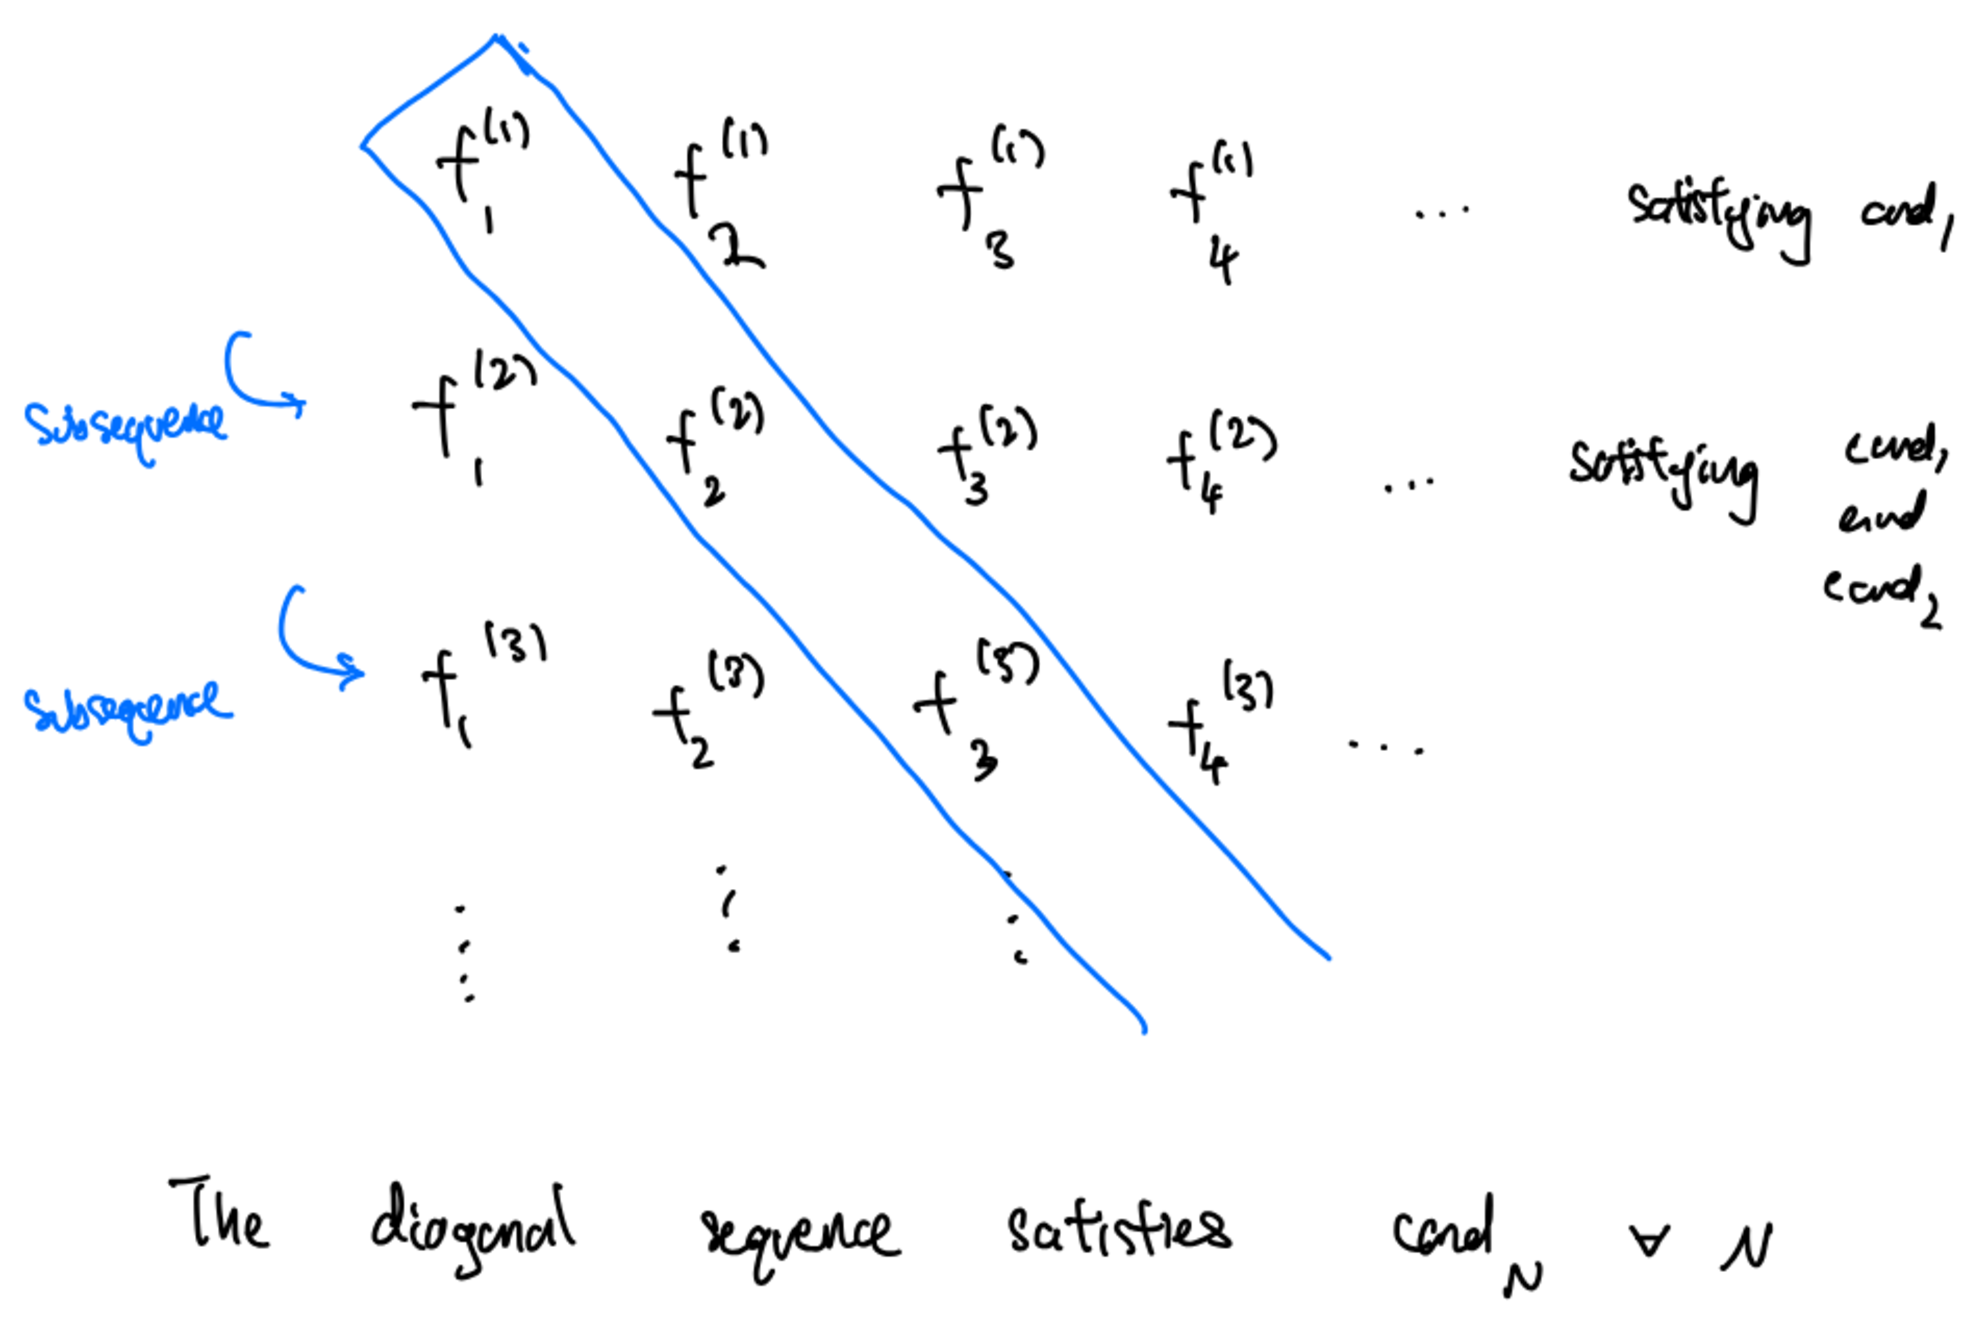
\includegraphics[scale = .2]{1.pdf}
    
\end{center}

Firstly we write \( U \) as a rising union of compact sets. 
\[
    U = \bigcup_{n=1}^{\infty} K_{n}  \text{ where } K_{n} \subset \text{ interior}(K_{n + 1} ) 
\]


Then for any compact \( K \) we have that 
\[
    K \subset \bigcup_{n=1}^{\infty} K_{n} \subset \bigcup_{n=1}^{\infty} \text{ interior}(K_{n + 1} )
\]

this implies \( K \subset K_{n}  \) 

Now let's rename \( K_{n} = K  \). From here choose a countable set of dense points \( \left\{ z_{i}  \right\}  \)  in \( K_{n}  \). Let \( f_{i}  \)  be a sequence in \( \mathcal{F}  \). For each \( z_{i}  \)  consider \( \left\{ f_{i} (z_{1} ) \right\}_{i}   \), since we have a uniformly bounded condition there is a subsequence which converges. Now we let \( \text{cond}_n = \left\{ f_{m} (z_{n} ) \right\} \), which is convergent. After diagonalizing there exists a subsequence which converges at each \( z_{n}  \). 

Now we need to prove that \( f_{m_1}, f_{m_2}, \dots    \) converges uniformly on \( K \). Let \( \epsilon > 0 \) be given. Since \( \left\{ z_{n}  \right\}  \) is dense, for any \( z \in K \), \( \exists z_{n}  \) such that \( \left\lvert z - z_{n}  \right\rvert < \delta  \). 

\begin{align*}
    \left\lvert f_{m_{j} }(z) - f _{m_{j'}}(z) \right\rvert \leq \left\lvert f_{m_{j} }(z) - f_{m_{j} }(z_{n} )   \right\rvert + \left\lvert f_{m_{j} }(z_{n} ) - f_{m_{j'} }(z_{n} )   \right\rvert +  \left\lvert f_{m_{j'} }(z_{n} ) - f_{m_{j'} }(z )   \right\rvert < \epsilon  
\end{align*}
Since \( K \) is compact, \( \exists  \) finitely many \( B_\delta (z_{n} ) \) covering \( K \). The sequence \( f_{m_1}, f_{m_2}, \dots    \) converges at each \( z_{n}  \) which implies it converges uniformly at finitely many \( z_{n}  \). 
\end{proof}

\end{thrm}

\begin{thrm}{Montel's Theorem}{}
Let \( \mathcal{F}  \) be a family of holomorphic functions on \( U \), which is uniformly bounded on all compact subsets of \( U \). Then \( \mathcal{F}  \) is equicontinuous, hence (by Arzela-Ascoli) it is a normal family. 

\tcbline 

PANORAMA:
\begin{enumerate}[]
    \item It suffices show that the set of derivatives of the functions in the family \( \mathcal{F}  \) is uniformly bounded on compact subsets. 
    \item First we create a compact superset of some original compact set \( K \) with some buffer of say \( \delta  \), and lets called it \( K_\delta  \). Essentially the point is for this new set to include a ball of this buffer size for every point in it. 
    \item After this we now work in \( K_\delta  \). We first relate the equicontinuous condition to the integral of \( f \) using the fundamental theorem of calculus. Then we bound the integral using Cauchy's inequality.
    \item After bounding the estimate that Cauchy's inequality provides using the fact that \( f \) is uniformly bounded on compact subsets we are done. 
\end{enumerate}

\quad 

\begin{proof}
    It suffices show that the set of derivatives of the functions in the family \( \mathcal{F}  \) is uniformly bounded on compact subsets. Take some compact subset \( K \subset U \). Clearly \( \mathrm{dist}(K, \partial U) > 3\delta > 0  \) since \( U \) is open. So take some compact \( K \subset K_\delta  \)  such that \( B_\delta (z) \subset K_\delta \ \forall z \in K\).  
    Observe that we have that,
    \[
        |f(z_1) - f(z_2)| \leq \left\lvert \int _{z_1}^{z_2} f'(z) dz\right\rvert \leq |z_{1}- z_2 |\sup \left\lvert f'(z) \right\rvert .
    \]

    From Cauchy's inequality and the fact that the function is uniformly bounded on compact subsets we have
    \[
        |f'(z)| \leq \frac{1}{\delta }\sup _{w\in \partial B_\delta (z)} |f(z)| \leq B_{K_\delta }. 
    \]
    Since \( \partial B_\delta (z) \subset K_\delta  \), this implies the family is equicontinuous, hence, we are done. 
\end{proof}

\end{thrm}

\begin{thrm}{Riemann Mapping Theorem}{}
Suppose we have some set \( U \subsetneq \mathbb{C}  \) which is connected and simply connected. Let \( z_0 \in U \). Then there is a unique biholomorphism \( f: U \to \mathbb{D}  \) such that \( f(z_0) = 0 \) and \( f'(z_0)>0 \). 
\tcbline
As an aside let us recall some definitions. A set is \emph{connected} if it cannot be divided into two non-empty disjoint open sets, or if the only subsets which are both closed and open are the original set and the empty set. A set is \emph{simply connected } if there is a path joining any two points in the set, and if any path between the same two end points are homotopic. Basically any loop can be contracted to a point.     
\end{thrm}

From here let us consider a \( \mathcal{F} : \left\{ f:\Omega \to \mathbb{D}  \right\}  \), where each function is holomorphic, injective, and \( f(z_0) = 0 \). 

\begin{misc}{Proposition}{}
Let \( U \subset \mathbb{C}  \) be an open and connected set, and \( \left\{ f_{n} :U\to \mathbb{C}  \right\}_{n = 1}^{\infty}   \) be a sequence of injective holomorphic functions, converging uniformly to \( f\) on compact subsets. Then \( f \) is either injective or constant.
\tcbline
PANORAMA:
\begin{enumerate}[]
    \item The idea is to use the argument principle to count preimages. 
    \item We then assume for the sake of contradiction that \( f \)  is not injective and nonconstant. We then use this assumption of noninjectivity to create a difference function using one the two distinct points which breaks injectivity, we set it to be is zero at these points. However, we compare it to the sequence of functions we are given and after apply the argument principle and taking limits a contradiction arises. 
\end{enumerate}

\quad

\begin{proof}

    Suppose \( f \) is not injective. Then we have that \( \exists z_1 \neq z_2 \in U \), such that \( f(z_1) = f(z_2) \). Consider \( g_{n} (z)\coloneqq f_{n} (z) - f_{n} (z_2) \). Then \( g(z) \coloneqq \lim_{n \to \infty} g_{n} (z) = f(z )- f(z_2) \) has a zero at \( z_1 \). If \( g(z) \)  nonconstant, then zeros are isolated which implies \( |g(z)|\neq 0 \)  on \( \overline{B} _\epsilon (z_1) \setminus \left\{ z_1 \right\}  \) for some \( \epsilon >0 \). This further implies the following 
    \[
       0 = \lim_{n \to \infty} \frac{1}{2\pi i} \int _{\partial B_{\epsilon })z_1 }\frac{g_{n} '(z)}{g_{n} (z)}dz =   \frac{1}{2\pi i}\int _{\partial B_{\epsilon }(z_1) }\frac{g'(z)}{g(z)} dz \in \mathbb{Z} _{\geq 1}
    \]
    However, this implies \( f_{n} (z) - f(z_2) \) has a zero at \( z_1 \) for all large enough \( n \). This contradicts our initial assumption of these functions being injective. Hence, \( f \) is a constant or injective. 
\end{proof}

\end{misc}

\begin{thrm}{Riemann Mapping Theorem}{}
    Suppose we have some set \( U \subsetneq \mathbb{C}  \) which is connected and simply connected. Let \( z_0 \in U \). Then there is a unique biholomorphism \( f: U \to \mathbb{D}  \) such that \( f(z_0) = 0 \) and \( f'(z_0)>0 \). 
    \tcbline
PANORAMA:
\begin{enumerate}[]
    \item Step 1 is to find a injective holomorphic map, use the \( \log _{U}  \) function and translations and scalars to do this. Take some function of the form \( F(z) = \frac{1}{\log _{U} (z) - z_0} \). 
\end{enumerate}

\quad 

\begin{proof}
    Step 1 is to find an injective holomorphic map: 
    \begin{align*}
        U &\to  \Omega  \ \substack{\subset\\ \text{open}  } \ \mathbb{D} \\
        z_0 &\to 0
    \end{align*}
    By translating we may assume \( 0 \notin U \). By scaling we may assume \( z_0 = 1 \). Since \( U \) is simply connected there exists a \( \log _U(z) \) such that \( e^{\log _{u} (z)}  = z\). Now we now that \( \log _{U}  \)  is injective and because of this \( \log _{U} (z) \neq 2\pi i \ \  \forall z \in U\). This is because \( z_1 = e^{\log _U(z_1)} = e^{\log _U(z_2)} = z_2  \). Furthermore, as a consequence we have that \( \left\lvert \log _{U} (z) - 2\pi i \right\rvert  \) is bounded away from 0, hence \( F(z) = \frac{1}{\log _{U} (z)- 2\pi i} \) is bounded and injective. So we can scale and translate it, so it is contained in \( \mathbb{D}  \) and sends \( 1 \to  0 \).

    Step 2:

    Now consider some family \( \mathcal{F}   = \left\{ f:\Omega \to \mathbb{D} : f(0)= 0, f'(0)>0,  f \text{ holomorphic and injective}  \right\}  \). Since \( \mathcal{F} \) is uniformly bounded, \( \left\{ |f'(0)| \right\}_{f \in \mathcal{F} }  \) is bounded as well. Let \( C = \sup _{f\in \mathcal{F} }|f'(0)| \) and take \( f1,f_2, \dots \in \mathcal{F}  \) such that
    \[
        \lim_{n \to \infty} |f_n'(0)| = C.
    \] 
    By Montel's theorem there exists a convergent subsequence with holomorphic limit \( f \)  (since convergence is uniform on compact subsets). We have that \( f(0) = 0 \) and that \( f \) is injective from the preceding proposition since we have \( f'(0) = C > 0 \). 

    Step 3:

    We now claim that \( f \) is surjective. We will use the following: for \( \alpha  \in \mathbb{D}  \), 
    \[
        \gamma _\alpha (z) = \frac{\alpha - z}{1 - \overline{\alpha }z } 
    \]
    which is an automorphism of \( \mathbb{D}   \) exchanging \( 0 \leftrightarrow \alpha  \). In fact \( \gamma _\delta \circ \gamma _\delta = \mathrm{Id}  \).
\end{proof}

\end{thrm}


\end{document}